\BourbakiFrontChapter{INTRODUCTION}

Most branches of mathematics involve structures of a type different from the algebraic structures (groups, rings, fields, etc.) which are the subject of the book Algebra of this series: namely structures which give a mathematical content to the intuitive notions of limit, continuity and neighbourhood. These structures are the subject matter of the present book.

Historically, the ideas of limit and continuity appeared very early in mathematics, notably in geometry, and their role has steadily increased with the development of analysis and its applications to the experimental sciences, since these ideas are closely related to those of experimental determination and approximation. But since most experimental determinations are measurements, that is to say determinations of one or more numbers, it is hardly surprising that the notions of limit and continuity in mathematics were featured at first only in the theory of real numbers and its outgrowths and fields of application (complex numbers, real or complex functions of real or complex variables, Euclidean geometry and related geometries).

In recent times it has been realized that the domain of applicability of these ideas far exceeds the real and complex numbers of classical analysis (see the Historical Note to Chapter I). Their essential content has been extracted by an effort of analysis and abstraction, and the result is a tool whose usefulness has become apparent in many branches of mathematics.

In order to bring out what is essential in the ideas of limit, continuity and neighbourhood, we shall begin by analysing the notion of neighbourhood (although historically it appeared later than the other two). If we start from the physical concept of approximation, it is natural to say that a subset A of a set E is a neighbourhood of an element a of A if, whenever we replace a by an element that ``approximates'' a, this new element will also belong to A, provided of course that the ``error'' involved is small enough; or, in other words, if all the points of E which are ``sufficiently near'' a belong to A. This definition is meaningful whenever precision can be given to the concept of sufficiently small error or of an element sufficiently near another. In this direction, the first idea was to suppose that the ``distance'' between two elements can be measured by a (positive) real number. Once the ``distance'' between any two elements of a set has been defined, it is clear how the ``neighbourhoods'' of an element a should be defined: a subset will be a neighbourhood of a if it contains all elements whose distance from a is less than some preassigned strictly positive number. Of course, we cannot expect to develop an interesting theory from this definition unless we impose certain conditions or axioms on the ``distance'' (for example, the inequalities relating the distances between the three vertices of a triangle which hold in Euclidean geometry should continue to hold for our generalized distance). In this way we arrive at a vast generalization of Euclidean geometry. It is convenient to continue to use the language of geometry: thus the elements or a set on which a ``distance'' has been defined are called points, and the set itself is called a space. We shall study such spaces in Chapter IX.

So far we have not succeeded in freeing ourselves from the real numbers. Nevertheless, the spaces so defined have a great many properties which can be stated without reference to the ``distance'' which gave rise to them. For example, every subset which contains a neighbourhood of a is again a neighbourhood of a, and the intersection of two neighbourhoods of a is a neighbourhood of a. These properties and others have a multitude of consequences which can be deduced without any further recourse to the ``distance'' which originally enabled us to define neighbourhoods. We obtain statements in which there is no mention of magnitude or distance.

We are thus led at last to the general concept of a topological space, which does not depend on any preliminary theory of the real numbers. We shall say that a set E carries a topological structure whenever we have associated with each element of E, by some means or other, a family of subsets of E which are called neighbourhoods of this element --- provided of course that these neighbourhoods satisfy certain conditions (the axioms of topological structures). Evidently the choice of axioms to be imposed is to some extent arbitrary, and historically has been the subject of a great deal of experiment (see the Historical Note to Chapter I). The system of axioms finally arrived at is broad enough for the present needs of mathematics, without falling into excessive and pointless generality.

A set carrying a topological structure is called a topological space and its elements are called points. The branch of mathematics which studies topological structures bears the name of Topology (etymologically, ``science of place'', not a particularly expressive name), which is preferred nowadays to the earlier (and synonymous) name of Analysis situs.

To formulate the idea of neighbourhood we started from the vague concept of an element ``sufficiently near'' another element. Conversely, a topological structure now enables us to give precise meaning to the phrase ``such and such a property holds for all points sufficiently near a'': by definition this means that the set of points which have this property is a neighbourhood of a for the topological structure in question.

From the notion of neighbourhood there flows a series of other notions whose study is proper to topology: the interior of a set, the closure of a set, the frontier of a set, open sets, closed sets, and so on (see Chapter I, § 1). For example, a subset A is an open set if, whenever a point \(a\) belongs to A, all the points sufficiently near \(a\) belong to A; in other words, if A is a neighbourhood of each of its points. The axioms for neighbourhoods have certain consequences for all these notions; for example, the intersection of two open sets is an open set (because we have supposed that the intersection of two neighbourhoods of \(a\) is a neighbourhood of \(a\) ). Conversely, we can start from one of these derived notions instead of starting from the notion of a neighbourhood; for example, we may suppose that the open sets are known, and take as axioms the properties of the family of open sets (one of these properties has just been stated, by way of example). We can then verify that, from knowledge of the open sets, the neighbourhoods can be reconstructed; the axioms for neighbourhoods are now consequences of the new axioms for open sets that we took as a starting point. Thus a topological structure can be defined in various different ways which are basically equivalent. In this book we shall start from the notion of open set, because the corresponding axioms are the simplest.

Once topological structures have been defined, it is easy to make precise the idea of continuity. Intuitively, a function is continuous at a point if its value varies as little as we please whenever the argument remains sufficiently near the point in question. Thus continuity will have an exact meaning whenever the space of arguments and the space of values of the function are topological spaces. The precise definition is given in Chapter I, § 2.

As with continuity, the idea of a limit involves two sets, each endowed with suitable structures, and a mapping of one set into the other. For example, the limit of a sequence of real numbers \(a_{n}\) involves the set N of natural numbers, the set R of real numbers, and a mapping of the former set into the latter. A real number a is then said to be a limit of the sequence if, whatever neighbourhood V of a we take, this neighbourhood contains all the \(a_{n}\) except for a finite number of values of n; that is, if the set of natural numbers n for which \(a_{n}\) belongs to V is a subset of N whose complement is finite. Note that R is assumed to carry a topological structure, since we are speaking of neighbourhoods; as to the set N, we have made a certain family of subsets play a particular part, namely those subsets whose complement is finite. This is a general fact: whenever we speak of limit, we are considering a mapping \(f\) of a set \(\mathbf{E}\) into a topological space \(\mathbf{F}\) , and we say that \(f\) has a point \(a\) of \(\mathbf{F}\) as a limit if the set of elements \(x\) of \(\mathbf{E}\) whose image \(f(x)\) belongs to

a neighbourhood V of a {[}this set is just the ``inverse image'' \(\overline{f}^{1}(V)\) {]} belongs, whatever the neighbourhood V, to a certain family F of subsets of E, given beforehand. For the notion of limit to have the essential properties ordinarily attributed to it, the family F must satisfy certain axioms, which are stated in Chapter I, § 6. Such a family F of subsets of E is called a filter on E. The notion of a filter, which is thus inseparable from that of a limit, appears also in other contexts in topology; for example, the neighbourhoods of a point in a topological space form a filter.

The general study of all these notions is the essential purpose of Chapter I. In addition, particular classes of topological spaces are considered there, spaces which satisfy more restrictive axioms, or spaces obtained by particular procedures from other given spaces.

As we have already said, a topological structure on a set enables one to give an exact meaning to the phrase ``whenever x is sufficiently near a, x has the property \(P\{x\}\) ''. But, apart from the situation in which a ``distance'' has been defined, it is not clear what meaning ought to be given to the phrase ``every pair of points x, y which are sufficiently near each other has the property \(P\{x, y\}\) '', since a priori we have no means of comparing the neighbourhoods of two different points. Now the notion of a pair of points near to each other arises frequently in classical analysis (for example, in propositions which involve uniform continuity). It is therefore important that we should be able to give a precise meaning to this notion in full generality, and we are thus led to define structures which are richer than topological structures, namely uniform structures. They are the subject of Chapter II.

The other chapters of this Book are devoted to questions in which, in addition to a topological or uniform structure, there is some other structure present. For example a group which carries a suitable topology (compatible in a certain sense with the group structure) is called a topological group. Topological groups are studied in Chapter III, and we shall see there in particular how every topological group can be endowed with certain uniform structures.

In Chapter IV we apply the preceding principles to the field of rational numbers. This enables us to define the field of real numbers; because of its importance, we study it in considerable detail. In the succeeding chapters, starting from the real numbers, we define certain topological spaces which are of particular interest in applications of topology to classical geometry: finite-dimensional vector spaces, spheres, projective spaces, etc. We consider also certain topological groups closely related to

the additive group of real numbers, which we characterize axiomatically, and this leads us to the definition and elementary properties of the most important functions of classical analysis: the exponential, logarithmic and trigonometric functions.

In Chapter IX we revert to general topological spaces, but now with a new instrument, namely the real numbers, at our disposal. In particular we study spaces whose topology is defined by means of a ``distance''; these spaces have properties, some of which cannot be extended to more general spaces. In Chapter X we study sets of mappings of a topological space into a uniform space (function spaces); these sets, suitably topologized, have interesting properties which already play an important part in classical analysis.

\chapter{Topological Structures}

\section{OPEN SETS, NEIGHBOURHOODS, CLOSED SETS}

\subsection{OPEN SETS}

DEFINITION 1. A topological structure (or, more briefly, a topology) on a set X is a structure given by a set D of subsets of X, having the following properties (called axioms of topological structures):

\((\mathbf{O}_{\mathbf{I}})\) Every union of sets of \(\mathfrak{D}\) is a set of \(\mathfrak{D}\) .

\((\mathbf{O}_{\mathbf{II}})\) Every finite intersection of sets of \(\mathfrak{D}\) is a set of \(\mathfrak{D}\) .

The sets of \(\mathfrak{D}\) are called open sets of the topological structure defined by \(\mathfrak{D}\) on \(\mathbf{X}\) .

DEFINITION 2. A topological space is a set endowed with a topological structure.

The elements of a topological space are often called points. When a topology has been defined on a set X, this set is said to be the set underlying the topological space X.

Axiom \((\mathrm{O}_{\mathrm{I}})\) implies in particular that the union of the empty subset of D, i.e.~the empty set belongs to D. Axiom \((\mathrm{O}_{\mathrm{II}})\) implies that the intersection of the empty subset of D, i.e.~the set X, belongs to D.

Examples of topologies. Given any set X, the set of subsets of X consisting of X and \(\varnothing\) satisfies axioms \((\mathrm{O}_{\mathrm{I}})\) and \((\mathrm{O}_{\mathrm{II}})\) and therefore defines a topology on X. So does the set \(\mathfrak{P}(\mathbf{X})\) of all subsets of X: the topology it defines is the discrete topology on X, and the set X with this topology is called a discrete space.

A covering \((\mathbf{U}_i)_{i\in I}\) of a subset \(\mathbf{A}\) of a topological space \(\mathbf{X}\) is said to be open if all the \(\mathbf{U}_i\) are open in \(\mathbf{X}\) .

DEFINITION 3. A homeomorphism of a topological space X onto a topological space X' is an isomorphism of the topological structure of X onto that of X'; that is to say, in accordance with the general definitions a bijection of X onto X' which transforms the set of open subsets of X into the set of open subsets of X'.

X and \(X'\) are said to be homeomorphic if there is a homeomorphism of X onto \(X'\) .

Example. If X and \(X'\) are two discrete spaces, any bijection of X onto \(X'\) is a homeomorphism.

The following criterion follows immediately from the definition of a homeomorphism: for a bijection \(f\) of a topological space \(\mathbf{X}\) onto a topological space \(\mathbf{X}'\) to be a homeomorphism, it is necessary and sufficient that the image under \(f\) of each open set in \(\mathbf{X}\) is an open set in \(\mathbf{X}'\) , and that the inverse image under \(f\) of each open set in \(\mathbf{X}'\) is an open set in \(\mathbf{X}\) .

\subsection{NEIGHBOURHOODS}

DEFINITION 4. Let X be a topological space and A any subset of X. A neighbourhood of A is any subset of X which contains an open set containing A. The neighbourhoods of a subset \(\{x\}\) consisting of a single point are also called neighbourhoods of the point x.

It is clear that every neighbourhood of a subset A of X is also a neighbourhood of each subset \(B \subset A\) ; in particular, it is a neighbourhood of each point of A. Conversely, suppose A is a neighbourhood of each of the points of a set B, and let U be the union of the open sets contained in A; then \(U \subset A\) , and since each point of B belongs to an open set contained in A, we have \(B \subset U\) ; but U is open by virtue of \((\mathrm{O}_{\mathrm{I}})\) , hence A is a neighbourhood of B. In particular:

PROPOSITION 1. A set is a neighbourhood of each of its points if and only if it is open.

The everyday sense of the word ``neighbourhood'' is such that many of the properties which involve the mathematical idea of neighbourhood appear as the mathematical expression of intuitive properties; the choice of this term thus has the advantage of making the language more expressive. For this purpose it is also permissible to use the expressions ``sufficiently near'' and ``as near as we please'' in some statements. For example, Proposition 1 can be stated in the following form: a set A is open if and only if, for each \(x \in A\) , all the points sufficiently near x belong to A. More generally, we shall say that a property holds for all points sufficiently near a point x, if it holds at all points of some neighbourhood of x.

Let us denote by \(\mathfrak{B}(x)\) the set of all neighbourhoods of \(x\) . The sets \(\mathfrak{B}(x)\) have the following properties:

\((\mathbf{V}_{\mathbf{I}})\) Every subset of \(\mathbf{X}\) which contains a set belonging to \(\mathfrak{B}(x)\) itself belongs to \(\mathfrak{B}(x)\) .

\((V_{II})\) Every finite intersection of sets of \(\mathfrak{B}(x)\) belongs to \(\mathfrak{B}(x)\) .

\((V_{\mathrm{III}})\) The element \(x\) is in every set of \(\mathfrak{B}(x)\) .

Indeed, these three properties are immediate consequences of Definition 4 and axiom (O \(_{II}\) ).

\((V_{IV})\) If V belongs to \(\mathfrak{B}(x)\) , then there is a set W belonging to \(\mathfrak{B}(x)\) such that, for each \(y \in W\) , V belongs to \(\mathfrak{B}(y)\) .

By Proposition 1, we may take W to be any open set which contains x and is contained in V.

This property may be expressed in the form that a neighbourhood of x is also a neighbourhood of all points sufficiently near to x.

These four properties of the sets \(\mathfrak{B}(x)\) are characteristic. To be precise, we have:

PROPOSITION 2. If to each element \(x\) of a set \(\mathbf{X}\) there corresponds a set \(\mathfrak{B}(x)\) of subsets of \(\mathbf{X}\) such that the properties \((\mathbf{V}_{\mathbf{I}}), (\mathbf{V}_{\mathbf{II}}), (\mathbf{V}_{\mathbf{III}})\) and \((\mathbf{V}_{\mathbf{IV}})\) are satisfied, then there is a unique topological structure on \(\mathbf{X}\) such that, for each \(x \in \mathbf{X}\) , \(\mathfrak{B}(x)\) is the set of neighbourhoods of \(x\) in this topology.

By Proposition 1, if there is a topology on X satisfying these conditions, the set of open sets for this topology is necessarily the set \(\mathfrak{D}\) of subsets A of X such that for each \(x \in \mathbf{A}\) we have \(\mathbf{A} \in \mathfrak{B}(x)\) ; hence the uniqueness of this topology if it exists.

The set \(\mathfrak{D}\) certainly satisfies axioms \((\mathrm{O_I})\) and \((\mathrm{O_{II}})\) : for \((\mathrm{O_I})\) , this follows immediately from \((\mathrm{V_I})\) , and for \((\mathrm{O_{II}})\) , from \((\mathrm{V_{II}})\) . It remains to show that, in the topology defined by \(\mathfrak{D}\) , \(\mathfrak{B}(x)\) is the set of neighbourhoods of \(x\) for each \(x \in \mathbf{X}\) . It follows from \((\mathbf{V}_{\mathbf{I}})\) that every neighbourhood of \(x\) belongs to \(\mathfrak{B}(x)\) . Conversely, let \(\mathbf{V}\) be a set belonging to \(\mathfrak{B}(x)\) , and let \(\mathbf{U}\) be the set of points \(y \in \mathbf{X}\) such that \(\mathbf{V} \in \mathfrak{B}(y)\) ; if we can show that \(x \in \mathbf{U}\) , \(\mathbf{U} \subset \mathbf{V}\) and \(\mathbf{U} \in \mathfrak{D}\) , then the proof will be complete. We have \(x \in \mathbf{U}\) since \(\mathbf{V} \in \mathfrak{B}(x)\) ; also \(\mathbf{U} \subset \mathbf{V}\) , for every point \(y \in \mathbf{U}\) belongs to \(\mathbf{V}\) by reason of \((\mathbf{V}_{\mathbf{III}})\) and the hypothesis \(\mathbf{V} \in \mathfrak{B}(y)\) . It remains to show that \(\mathbf{U} \in \mathfrak{D}\) , i.e.~that \(\mathbf{U} \in \mathfrak{B}(y)\) for each \(y \in \mathbf{U}\) ; now (Fig. 1) if \(y \in \mathbf{U}\) then by \((\mathbf{V}_{\mathbf{IV}})\) there is a set \(\mathbf{W}\) such that for each \(z \in \mathbf{W}\) we have \(\mathbf{V} \in \mathfrak{B}(z)\) ; since \(\mathbf{V} \in \mathfrak{B}(z)\) means that \(z \in \mathbf{U}\) , it follows that \(\mathbf{W} \subset \mathbf{U}\) , and therefore, by \((\mathbf{V}_{\mathbf{I}})\) , that \(\mathbf{U} \in \mathfrak{B}(y)\) . Q.E.D.

\pandocbounded{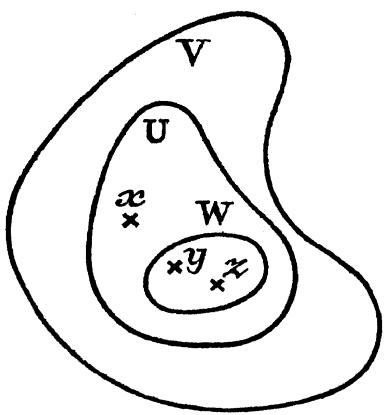
\includegraphics[keepaspectratio]{images/part001_56c83e78.jpg}}\\
Figure 1.

Proposition 2 shows that a topology on X can be defined by means of the sets \(\mathfrak{B}(x)\) of neighbourhoods of points of X, subject only to the axioms \((\mathrm{V}_{\mathrm{I}})\) , \((\mathrm{V}_{\mathrm{II}})\) , \((\mathrm{V}_{\mathrm{III}})\) and \((\mathrm{V}_{\mathrm{IV}})\) .

Example. We may define a topology on the set \(\mathbf{Q}\) of rational numbers by taking for open sets all unions of bounded open intervals; the set of these subsets certainly satisfies \((\mathrm{O}_{\mathbf{I}})\) , and to see that it satisfies \((\mathrm{O}_{\mathbf{II}})\) it is enough to remark that if the intersection of two open intervals \(]a, b[\) and \(]c, d[\) is not empty, then it is the interval \(]\alpha, \beta[\) , where \(\alpha = \sup (a, c)\) and \(\beta = \inf (b, d)\) . We get the same topology by defining for each \(x \in \mathbf{Q}\) the set \(\mathfrak{B}(x)\) of neighbourhoods of \(x\) to be the set of subsets containing an open interval to which \(x\) belongs. The topological space obtained by assigning this topology to \(\mathbf{Q}\) is called the rational line (cf.~Chapter IV, § 1, no. 2). Notice that in this space every open interval is an open set. * We can define a topology on the set \(\mathbf{R}\) of real numbers in the same way; \(\mathbf{R}\) with this topology is called the real line (cf.~§ 2, Exercise 5 and Chapter IV, § 1, no. 3). *

\subsection{FUNDAMENTAL SYSTEMS OF NEIGHBOURHOODS; BASES OF A TOPOLOGY}

DEFINITION 5. In a topological space X, a fundamental system of neighbourhoods of a point x (resp. of a subset A of X) is any set S of neighbourhoods of x (resp. A) such that for each neighbourhood V of x (resp. A) there is a neighbourhood W ∈ S such that W ⊂ V.

If \(\mathfrak{S}\) is a fundamental system of neighbourhoods of a subset \(A\) of \(X\) , then every finite intersection of sets of \(\mathfrak{S}\) contains a set of \(\mathfrak{S}\) .

Examples. 1) In a discrete space (no. 1) the set \(\{x\}\) alone constitutes a fundamental system of neighbourhoods of the point \(x\) .

\begin{enumerate}
\def\labelenumi{\arabic{enumi})}
\setcounter{enumi}{1}
\tightlist
\item
  On the rational line Q the set of all open intervals containing a point x is a fundamental system of neighbourhoods of this point. So is the set of open intervals \(]x - 1/n, x + 1/n[\) , and the set of closed intervals \([x - 1/n, x + 1/n]\) , where n runs through all the integers \textgreater0, or through any infinite strictly increasing sequence of integers \textgreater0. * There are analogous results for the real line. *
\end{enumerate}

DEFINITION 6. A base of the topology of a topological space X is any set B of open subsets of X such that every open subset of X is the union of sets belonging to B.

PROPOSITION 3. If X is a topological space, then for a set B of open subsets of X to be a base of the topology of X it is necessary and sufficient that for each \(x \in X\) the set of \(V \in B\) such that \(x \in V\) is a fundamental system of neighbourhoods of x.

It is clear that the condition is necessary. Conversely, if it is satisfied, then given any open set U and any \(x \in U\) there is an open set \(V_{x} \in B\) such that \(x \in V_{x} \subset U\) . The union of the sets \(V_{x}\) for \(x \in U\) is therefore equal to U. This completes the proof.

Examples. 1) The discrete topology has as a base the set of subsets of X which consist of a single point.

\begin{enumerate}
\def\labelenumi{\arabic{enumi})}
\setcounter{enumi}{1}
\tightlist
\item
  The set of bounded open intervals is by definition a base of the topology of the rational line (no. 2). * Likewise, the set of bounded open intervals is a base of the topology of the real line. *
\end{enumerate}

\subsection{CLOSED SETS}

DEFINITION 7. In a topological space X, the complements of the open sets of X are called closed sets.

Taking complements, we find that the axioms \((\mathbf{O}_{\mathbf{I}})\) and \((\mathbf{O}_{\mathbf{II}})\) take the following form:

\((\mathbf{O}_{\mathbf{I}}^{\prime})\) Every intersection of closed sets is a closed set.

\((\mathbf{O}_{\mathrm{II}}^{\prime})\) Every finite union of closed sets is a closed set.

The empty set and the whole space X are closed (and therefore both open and closed; cf.~§ 11).

On the rational line, every interval of the form \([a, \rightarrow[\) is a closed set, for its complement \(]\leftarrow, a[\) is open; likewise, every interval of the form \(]\leftarrow, a]\) is a closed set; hence so is every bounded closed interval \([a, b]\) , since it is the intersection of the intervals \([a, \rightarrow[\) and \(]\leftarrow, b]\) .

The set Z of rational integers is closed in the rational line, since its

complement \(\bigcup_{n\in \mathbf{Z}}]n,n + 1[\) is open.

A covering \((\mathbf{F}_i)_{i\in I}\) of a subset \(\mathbf{A}\) of a topological space \(\mathbf{X}\) is said to be closed if each of the \(\mathbf{F}_i\) is closed in \(\mathbf{X}\) .

A homeomorphism \(f\) of a topological space \(\mathbf{X}\) onto a topological space \(\mathbf{X}'\) (no. 1) can be characterized as a bijection of \(\mathbf{X}\) onto \(\mathbf{X}'\) such that the image under \(f\) of every closed subset of \(\mathbf{X}\) is a closed subset of \(\mathbf{X}'\) and the inverse image under \(f\) of every closed subset of \(\mathbf{X}'\) is a closed subset of \(\mathbf{X}\) .

\subsection{LOCALLY FINITE FAMILIES}

DEFINITION 8. A family \((\mathbf{A}_{i})_{i\in \mathbf{I}}\) of subsets of a topological space \(\mathbf{X}\) is said to be locally finite if for each \(x\in \mathbf{X}\) there is a neighbourhood \(\mathbf{V}\) of \(x\) such that \(\mathbf{V}\cap \mathbf{A}_i = \emptyset\) for all but a finite number of indices \(i\in \mathbf{I}\) . A set \(\mathfrak{S}\) of subsets of \(\mathbf{X}\) is said to be locally finite if the family of subsets defined by the identity map of \(\mathfrak{S}\) onto itself is locally finite.

It is clear that if \((\mathbf{A}_t)_{t \in \mathbf{I}}\) is a locally finite family of subsets and if \(\mathbf{B}_t \subset \mathbf{A}_t\) for each \(t \in \mathbf{I}\) , then the family \((\mathbf{B}_t)_{t \in \mathbf{I}}\) is locally finite.

Every finite family of subsets of a topological space X is obviously locally finite; the converse is not true in general.

* For example, in R, the open covering formed by the interval \(]\leftarrow, 1[\) and the intervals \(]n, \rightarrow[\) for each integer \(n\geqslant0\) is locally finite; and each interval \(]n, \rightarrow[\) meets an infinite number of sets of this covering.

PROPOSITION 4. The union of a locally finite family of closed subsets of a topological space X is closed in X.

Let \((\mathbf{F}_i)_{i\in I}\) be a locally finite family of closed subsets of \(X\) , and suppose that \(x\in X\) does not belong to \(\mathbf{F} = \bigcup_{i\in I}\mathbf{F}_i\) ; then \(x\) has a neighbourhood \(V\) which meets only those \(\mathbf{F}_i\) whose indices belong to a finite subset \(J\) of \(I\) . For each \(i\in J\) let \(\mathbf{U}_i\) be the complement of \(\mathbf{F}_i\) ; then \(\mathbb{CF}\) contains the set \(V\cap \bigcap_{i\in J}\mathbf{U}_i\) , which is a neighbourhood of \(x\) since each \(\mathbf{U}_i\) is open and contains \(x\) . Hence, by Proposition 1 of no. 2, \(\mathbb{CF}\) is open and therefore \(\mathbf{F}\) is closed in \(X\) .

We note that the union of an arbitrary family of closed subsets of X is not necessarily closed; for example, on the rational line Q, the set \(]0, 1[\) is the union of the closed sets

\[
\left[ \frac {1}{n}, 1 - \frac {1}{n} \right] \quad \text { for } n > 2,
\]

but is not closed.

\subsection{INTERIOR, CLOSURE, FRONTIER OF A SET; DENSE SETS}

DEFINITION 9. In a topological space X, a point x is said to be an interior point of a subset A of X if A is a neighbourhood of x. The set of interior points of A is called the interior of A and is denoted by \(\mathring{A}\).

According to Definitions 9 and 4, a point x is an interior point of A if there is an open set contained in A which contains x; it follows that \(\mathring{A}\) is the union of all the open sets contained in A, and hence is the largest open set contained in A: in other words, if B is an open set contained in A, then B ⊂ \(\mathring{A}\). Consequently, if A and B are two subsets of X such that B ⊂ A, then \(\mathring{B} \subset \mathring{A}\); and A is a neighbourhood of B if and only if B ⊂ \(\mathring{A}\).

Remark. The interior of a non-empty set can be empty; this is the case for a set consisting of a single point which is not open, for example on the rational line * (or the real line) *.

Proposition 1 of no. 2 can be restated as follows:

A set is open if and only if it coincides with its interior.

The property \((V_{II})\) of no. 2 implies that every point which is an interior point of each of two subsets A and B is an interior point of \(A \cap B\) ; consequently

\[
\mathring {\mathbf {A} \cap \mathbf {B}} = \mathring {\mathbf {A}} \cap \mathring {\mathbf {B}}.\tag{1}
\]

Every point which is interior to the complement of a set A is said to be an exterior point of A, and the set of these points is called the exterior of A in X; a point \(x \in X\) which is an exterior point of A is therefore characterized by the property that x has a neighbourhood which does not meet A.

DEFINITION 10. The closure of a subset A of a topological space X is the set of all points \(x \in X\) such that every neighbourhood of x meets A, and is denoted by \(\overline{A}\) .

This definition can be reformulated by saying that a point x lies in the closure of a set A if there are points of A as near x as we please to.

Every point which is not in the closure of A is exterior to A, and conversely; thus we have the formulae (which are duals of each other)

\[
\mathbf {C} \overline {{\mathbf {A}}} = \mathring {\mathbf {C} \mathbf {A}}, \quad \mathbf {C} \mathring {\mathbf {A}} = \overline {{\mathbf {C} \mathbf {A}}}.\tag{2}
\]

Hence, to any proposition on interiors of sets, there corresponds by duality a proposition on closures, and vice versa. In particular, the closure of a set A is the smallest closed set which contains A; in other words, if B is a closed set such that \(A \subset B\) , then \(\overline{A} \subset B\) . If A and B are two subsets of X such that \(A \subset B\) , then \(\overline{A} \subset \overline{B}\) .

A set is closed if and only if it coincides with its closure.

The dual of formula (1) is

\[
\overline {{{\mathbf {A} \cup \mathbf {B}}}} = \overline {{{\mathbf {A}}}} \cup \overline {{{\mathbf {B}}}}.\tag{3}
\]

PROPOSITION 5. Let A be an open set in X; then for every subset B of X we have

\[
\mathbf {A} \cap \overline {{\mathbf {B}}} \subset \overline {{\mathbf {A} \cap \mathbf {B}}}.\tag{4}
\]

For suppose \(x \in A \cap \overline{B}\) ; then if V is any neighbourhood of x, \(V \cap A\) is a neighbourhood of x, since A is open; hence \(V \cap A \cap B\) is not empty and therefore x lies in the closure of \(A \cap B\) .

If \(x\) lies in the closure of \(A\) but not in \(A\) , then every neighbourhood of \(x\) contains a point of \(A\) other than \(x\) ; but if \(x \in A\) it can happen that \(x\) has a neighbourhood which contains no point of \(A\) except \(x\) . We say then that \(x\) is an isolated point of \(A\) . In particular, \(x\) is isolated in the whole space \(X\) if and only if \(\{x\}\) is an open set.

A closed set which has no isolated points is called a perfect set.

DEFINITION 11. In a topological space X, a point x is said to be a frontier point of a set A if x lies in the closure of A and in the closure of CA. The set of frontier points of A is called the frontier of A.

The frontier of A is therefore the set \(\overline{A} \cap \overline{\complement A}\) , which is closed. A frontier point x of A is characterized by the property that every neighbourhood of x contains at least one point of A and at least one point of CA; x may or may not belong to A. The frontier of A is the same as the frontier of CA. The interior of A, the exterior of A and the frontier of A are mutually disjoint and their union is the whole space X.

DEFINITION 12. A subset A of a topological space X is said to be dense in X (or simply dense, if there is no ambiguity about X) if \(\overline{A} = X\) , i.e.~if every non-empty open set U of X meets A.

Examples. * We shall see in Chapter IV, § 1 that the set of rational numbers and its complement are dense on the real line. *

In a discrete space X the only dense subset of X is \(X^{*}\) itself. On the other hand, every non-empty subset of X is dense in the topology on X for which the only open sets are \(\varnothing\) and X.

PROPOSITION 6. If \(\mathfrak{B}\) is a base of the topology of a topological space \(X\) , there is a dense set \(D\) in \(X\) such that \(\operatorname{Card}(D) \leqslant \operatorname{Card}(\mathfrak{B})\) .

We may restrict ourselves to the case in which none of the sets of \(\mathfrak{B}\) is empty (the non-empty sets of \(\mathfrak{B}\) already form a base of the topology of \(\mathbf{X}\) ). For each \(\mathbf{U} \in \mathfrak{B}\) , let \(x_{\mathbf{U}}\) be a point of \(\mathbf{U}\) ; it follows from Proposition 3 of no. 3 that the set \(\mathbf{D}\) of the points \(x_{\mathbf{U}}\) is dense in \(\mathbf{X}\) , and we have Card \((\mathbf{D}) \leqslant\) Card \((\mathfrak{B})\) (Set Theory, Chapter III, § 3, no. 2, Proposition 3).

\section{CONTINUOUS FUNCTIONS}

\subsection{CONTINUOUS FUNCTIONS}

DEFINITION 1. A mapping \(f\) of a topological space \(\mathbf{X}\) into a topological space \(\mathbf{X}'\) is said to be continuous at a point \(x_0 \in \mathbf{X}\) if, given any neighbourhood \(\mathbf{V}'\) of \(f(x_0)\) in \(\mathbf{X}'\) , there is a neighbourhood \(\mathbf{V}\) of \(x_0\) in \(\mathbf{X}\) such that the relation \(x \in \mathbf{V}\) implies \(f(x) \in \mathbf{V}'\) .

Definition 1 may be restated in the following more intuitive form: to say that \(f\) is continuous at the point \(x_0\) means that \(f(x)\) is as near as we please to \(f(x_0)\) whenever \(x\) is sufficiently near \(x_0\) .

The relation ``for each \(x \in V\) , \(f(x) \in V'\) '' is equivalent to \(f(V) \subset V'\) or again to \(V \subset \overline{f}^{1}(V')\) ; in view of the neighbourhood axiom \((V_{I})\) , we see that Definition 1 is equivalent to the following: \(f: X \to X'\) is said to be continuous at the point \(x_{0}\) if, for each neighbourhood \(V'\) of \(f(x_{0})\) in \(X'\) , \(\overline{f}^{1}(V')\) is a neighbourhood of \(x_{0}\) in X. Moreover, it is sufficient that \(\overline{f}^{1}(V')\) is a neighbourhood of \(x_{0}\) for each neighbourhood \(V'\) belonging to a fundamental system of neighbourhoods of \(f(x_{0})\) in \(X'\) (§ 1, no. 3).

PROPOSITION 1. Let \(f\) be a mapping of a topological space \(\mathbf{X}\) into a topological space \(\mathbf{X}'\) . If \(f\) is continuous at \(x\) , and if \(x\) lies in the closure of a subset \(A\) of \(X\) , then \(f(x)\) lies in the closure of \(f(A)\) .

Let \(\mathbf{V}'\) be a neighbourhood of \(f(x)\) in \(\mathbf{X}'\) . Since \(f\) is continuous at \(x\) , \(\overline{f}^1 (\mathbf{V}')\) is a neighbourhood of \(x\) in \(\mathbf{X}\) . Hence \(\overline{f}^1 (\mathbf{V}')\) meets \(\mathbf{A}\) , from which it follows that \(\mathbf{V}'\) meets \(f(\mathbf{A})\) , and therefore \(f(x)\) is in the closure of \(f(\mathbf{A})\) .

PROPOSITION 2. Let X, X', X'' be three topological spaces; let f be a mapping of X into X', continuous at x ∈ X; let g be a mapping of X' into X'', continuous at f(x). Then the composition h = g \(\circ\) f: X → X'' is continuous at x.

Let \(V''\) be a neighbourhood of \(h(x) = g(f(x))\) in \(X''\) . Since \(g\) is continuous at \(f(x)\) it follows that \(\overline{g}^1(V'')\) is a neighbourhood of \(f(x)\) in \(X'\) . But \(f\) is continuous at \(x\) , hence \(\overline{f}^1(\overline{g}^1(V'')) = \overline{h}^1(V'')\) is a neighbourhood of \(x\) in \(X\) , and therefore \(h\) is continuous at \(x\) .

DEFINITION 2. A mapping of a topological space X into a topological space X' is said to be continuous on X (or just continuous) if it is continuous at each point of X.

Examples. 1) The identity mapping of a topological space X onto itself is continuous.

\begin{enumerate}
\def\labelenumi{\arabic{enumi})}
\setcounter{enumi}{1}
\item
  A constant map of a topological space into a topological space is continuous.
\item
  Every mapping of a discrete space into a topological space is continuous.
\end{enumerate}

THEOREM 1. Let \(f\) be a mapping of a topological space \(X\) into a topological space \(X'\) . Then the following statements are equivalent:

\begin{enumerate}
\def\labelenumi{\alph{enumi})}
\item
  \(f\) is continuous in \(\mathbf{X}\) .
\item
  For every subset A of X, \(f(\overline{\mathrm{A}}) \subset \overline{f(\mathrm{A})}\) .
\item
  The inverse image under \(f\) of every closed subset of \(\mathbf{X}'\) is a closed subset of \(\mathbf{X}\) .
\item
  The inverse image under \(f\) of every open subset of \(\mathbf{X}'\) is an open subset of \(\mathbf{X}\) .
\end{enumerate}

We have already seen that a) implies b) (Proposition 1). To show that b) implies c), let \(\mathbf{F}'\) be a closed subset of \(\mathbf{X}'\) and let \(\mathbf{F} = \overline{f}^{1}(\mathbf{F}')\) ; then by hypothesis \(f(\overline{\mathbf{F}}) \subset \overline{f(\mathbf{F})} \subset \overline{\mathbf{F}}' = \mathbf{F}'\) , hence \(\overline{\mathbf{F}} \subset \overline{f}^{1}(\mathbf{F}') = \mathbf{F} \subset \overline{\mathbf{F}}\) , so that \(\mathbf{F} = \overline{\mathbf{F}}\) and \(\mathbf{F}\) is closed. By virtue of the relation \(\complement \overline{f}^{1}(A') = \overline{f}^{1}(\complement A')\) for every subset \(A'\) of \(X'\) , c) implies d). Finally, suppose that d) is satisfied. Let \(x\) be any point of \(X\) and let \(V'\) be any neighbourhood of \(f(x)\) in \(X'\) ; then there is an open set \(A'\) in \(X'\) for which

\[
f (x) \in \mathrm{A} ^ {\prime} \subset \mathrm{V} ^ {\prime}
\]

and hence \(x \in \overline{f}^1(\mathbf{A}') \subset \overline{f}^1(\mathbf{V}')\) . By hypothesis, \(\overline{f}^1(\mathbf{A}')\) is open in \(\mathbf{X}\) , so that \(\overline{f}^1(\mathbf{V}')\) is a neighbourhood of \(x\) in \(\mathbf{X}\) . Thus d) implies a).

Remarks. 1) Let \(\mathfrak{B}\) be a base (§ 1, no. 3) of the topology of \(\mathbf{X}'\) ; then for \(f: \mathbf{X} \to \mathbf{X}'\) to be continuous, it is necessary and sufficient that \(\overline{f}^1(\mathbf{U}')\) is open in \(\mathbf{X}\) for every \(\mathbf{U}' \in \mathfrak{B}\) .

Examples. Let \(a\) be any rational number. The mapping \(x \to a + x\) of the rational line \(\mathbf{Q}\) into itself is continuous on \(\mathbf{Q}\) , for the inverse image under this mapping of an open interval \(]b, c[\) is the open interval

\[
] b - a, c - a [.
\]

Likewise, the mapping \(x \to ax\) is continuous on \(\mathbf{Q}\) ; this is clear if \(a = 0\) , for then \(ax = 0\) for all \(x\) ; if \(a \neq 0\) then the inverse image under this mapping of the open interval \(]b, c[\) is the open interval with end-points \(b / a\) and \(c / a\) .

\pandocbounded{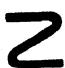
\includegraphics[keepaspectratio]{images/part001_4077020d.jpg}}

\begin{enumerate}
\def\labelenumi{\arabic{enumi})}
\setcounter{enumi}{1}
\tightlist
\item
  The direct image of an open (resp. closed) set of X under a continuous mapping \(f: \mathbf{X} \to \mathbf{X}'\) is not necessarily open (resp. closed) in \(\mathbf{X}'\) (cf.~§ 5).
\end{enumerate}

Example. * The mapping \(f: x \to 1 / (1 + x^2)\) of \(\mathbf{R}\) into itself is continuous, but \(f(\mathbf{R})\) is the half-open interval {[}0, 1{]}, which is neither open nor closed in \(\mathbf{R}\) . *

THEOREM 2. 1) If \(f: \mathbf{X} \to \mathbf{X}'\) and \(g: \mathbf{X}' \to \mathbf{X}''\) are two continuous mappings, then \(g \circ f: \mathbf{X} \to \mathbf{X}''\) is continuous.

\begin{enumerate}
\def\labelenumi{\arabic{enumi})}
\setcounter{enumi}{1}
\tightlist
\item
  For a bijection \(f\) of a topological space \(X\) onto a topological space \(X'\) to be a homeomorphism, it is necessary and sufficient that \(f\) and the inverse of \(f\) are continuous (or, as is also said, that \(f\) is bicontinuous).
\end{enumerate}

The first assertion is an immediate consequence of Proposition 2; the second follows from Theorem 1, d) and the definition of a homeomorphism (§ 1, no. 1).

\pandocbounded{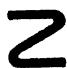
\includegraphics[keepaspectratio]{images/part001_720050f1.jpg}}

Remarks. 1) It is possible to have a continuous bijection of a topological space X onto a topological space X' which is not bicontinuous: for example, take X' to be the rational line Q, and X to be the set Q with the discrete topology; then the identity map X → X' is continuous but is not a homeomorphism.

\begin{enumerate}
\def\labelenumi{\arabic{enumi})}
\setcounter{enumi}{1}
\item
  To verify that a continuous bijection \(f: \mathbf{X} \to \mathbf{X}'\) is a homeomorphism, it is enough to show that for each \(x \in \mathbf{X}\) and each neighbourhood \(V\) of \(x\) , \(f(V)\) is a neighbourhood of \(f(x)\) in \(\mathbf{X}'\) .
\item
  Let X be a topological space, and for each \(x \in X\) let \(\mathfrak{B}(x)\) be the set of all neighbourhoods of x. Let \(x_{0}\) be a point of X; for each \(x \in X\) , define a set \(\mathfrak{B}_{0}(x)\) of subsets of X as follows: \(\mathfrak{B}_{0}(x_{0}) = \mathfrak{B}(x_{0})\) , and if \(x \neq x_{0}\) then \(\mathfrak{B}_{0}(x)\) is to be the set of all subsets of X which contain x. It is immediately verified (§ 1, no. 2, Proposition 2) that the sets \(\mathfrak{B}_{0}(x)\) are sets of neighbourhoods of points of X for a topology on X; let \(X_{0}\) denote the topological space thus obtained, and let \(j : X_{0} \to X\) denote the identity map, which is continuous but not in general bicontinuous. A mapping f of X into a topological space \(X'\) is continuous at the point \(x_{0}\) if and only if the composition \(X_{0} \stackrel{j}{\to} X \stackrel{f}{\to} X'\) is continuous on \(X_{0}\) ; this follows immediately from the definitions.
\end{enumerate}

\subsection{COMPARISON OF TOPOLOGIES}

Theorem 2 of no. 1 shows that we may take the continuous mappings as morphisms of topological structures (Set Theory, Chapter IV, § 2, no. 1); from now on, we shall assume that we have made this choice of morphisms. In accordance with the general definitions (Set Theory, Chapter IV, § 2, no. 2), this allows us to define an ordering on the set of topologies on a given set X:

DEFINITION 3. Given two topologies \(\mathfrak{C}_1\) , \(\mathfrak{C}_2\) on the same set X, we say that \(\mathfrak{C}_1\) is finer than \(\mathfrak{C}_2\) (and that \(\mathfrak{C}_2\) is coarser than \(\mathfrak{C}_1\) ) if, denoting by \(X_i\) the set X with the topology \(\mathfrak{C}_i\) ( \(i = 1, 2\) ), the identity mapping \(X_1 \to X_2\) is continuous. If in addition \(\mathfrak{C}_1 \neq \mathfrak{C}_2\) , we say that \(\mathfrak{C}_1\) is strictly finer than \(\mathfrak{C}_2\) (and that \(\mathfrak{C}_2\) is strictly coarser than \(\mathfrak{C}_1\) ).

Two topologies, one of which is finer than the other, are said to be comparable.

The criteria for a mapping to be continuous (no. 1, Definition 1 and Theorem 1) give the following proposition:

PROPOSITION 3. Given two topologies \(\mathfrak{G}_1\) , \(\mathfrak{G}_2\) on a set \(X\) , the following statements are equivalent:

\begin{enumerate}
\def\labelenumi{\alph{enumi})}
\item
  \(\mathfrak{C}_1\) is finer than \(\mathfrak{C}_2\) .
\item
  For each \(x \in \mathbf{X}\) , each neighbourhood of \(x\) for \(\mathfrak{C}_2\) is a neighbourhood of \(x\) for \(\mathfrak{C}_1\) .
\item
  For each subset A of X, the closure of A in the topology \(C_{1}\) is contained in the closure of A in the topology \(C_{2}\) .
\item
  Every subset of X which is closed in \(\mathfrak{C}_{2}\) is closed in \(\mathfrak{C}_{1}\) .
\item
  Every subset of X which is open in \(\mathfrak{C}_{2}\) is open in \(\mathfrak{C}_{1}\) .
\end{enumerate}

Example. * In Hilbert space H consisting of sequences \(x = (x_n)\) of real numbers such that

\[
\| x \| ^ {2} = \sum_ {n = 0} ^ {\infty} x _ {n} ^ {2} <   + \infty ,
\]

the neighbourhoods of a point \(x_0\) in the strong topology on H are the sets which contain an open ball \(\|x - x_0\| < a\) centred at \(x_0\) ; the neighbourhoods of \(x_0\) in the weak topology on H are the sets containing a set defined by relation of the form \(\sup_{1 \leqslant i \leqslant n} |(x - x_0|a_i)| \leqslant 1\) , where the \(a_i\) are points of H and

\[
(x | y) = \sum_ {n = 0} ^ {\infty} x _ {n} y _ {n}
\]

if \(x = (x_n)\) and \(y = (y_n)\) . Now if \(\beta = \sup_{1 \leqslant i \leqslant n} \|a_i\|\) , the relation \(\|x - x_0\| \leqslant 1/\beta\) implies that \(|(x - x_0|a_i)| \leqslant \|x - x_0\| \cdot \|a_i\| \leqslant 1\) for \(1 \leqslant i \leqslant n\) ; hence the strong topology on H is finer than the weak topology. On the other hand, given any finite family \((a_i)_{1 \leqslant i \leqslant n}\) of points of H, there are points \(x\) in H such that \((x - x_0|a_i) = 0\) for \(1 \leqslant i \leqslant n\) and such that \(\|x - x_0\|\) is arbitrarily large; this shows that the strong topology is strictly finer than the weak topology. *

Remarks. 1) In the ordered set of all topologies on a set X, the topology in which the only open sets are \(\varnothing\) and X is the coarsest and the discrete topology is the finest.

\begin{enumerate}
\def\labelenumi{\arabic{enumi})}
\setcounter{enumi}{1}
\item
  The finer the topology, the more open sets, closed sets and neighbourhoods; the finer the topology, the smaller (resp. the larger) the closure (resp. the interior) of a set; the finer the topology, the fewer dense sets.
\item
  If \(f: \mathbf{X} \to \mathbf{X}'\) is a continuous mapping, it remains continuous if the topology of \(\mathbf{X}\) is replaced by a finer topology and the topology of \(\mathbf{X}'\) is replaced by a coarser topology (no. 1, Theorem 2). In other words, the finer the topology of \(\mathbf{X}\) and the coarser the topology of \(\mathbf{X}'\) , the more continuous mappings there are of \(\mathbf{X}\) into \(\mathbf{X}'\) .
\end{enumerate}

\subsection{INITIAL TOPOLOGIES}

PROPOSITION 4. Let X be a set, let \((\mathbf{Y}_i)_{i \in I}\) be a family of topological spaces, and for each \(i \in I\) let \(f_i\) be a mapping of X into \(\mathbf{Y}_i\) . Let \(\mathfrak{S}\) be the set of subsets of X of the form \(\overline{f}_i^1 (\mathbf{U}_i)\) ( \(i \in I\) , \(\mathbf{U}_i\) open in \(\mathbf{Y}_i\) ), and let \(\mathfrak{B}\) be the set of finite intersections of sets of \(\mathfrak{S}\) . Then \(\mathfrak{B}\) is a base of a topology \(\mathfrak{C}\) on X which is the initial topological structure on X for the family \((f_i)\) (Set Theory, Chapter IV, § 2, no. 3) and in particular is the coarsest topology on X for which the mappings \(f_i\) are continuous. More precisely, if \(g\) is a mapping of a topological space Z into X, then \(g\) is continuous at a point \(z \in Z\) (X carrying the topology \(\mathfrak{C}\) ) if and only if each of the functions \(f_i \circ g\) is continuous at \(z\) .

Let \(\mathfrak{D}\) be the set of all unions of sets belonging to \(\mathfrak{B}\) ; clearly \(\mathfrak{D}\) satisfies axiom \((\mathrm{O}_{\mathrm{I}})\) since formation of unions is associative; and \(\mathfrak{D}\) satisfies axiom \((\mathrm{O}_{\mathrm{II}})\) by reason of the definition of \(\mathfrak{B}\) and the fact that finite intersection is distributive over arbitrary union {[}Set Theory, R § 4, formula (37){]}. The set \(\mathfrak{D}\) is therefore the set of open subsets of X for a topology \(\mathfrak{G}\) of which \(\mathfrak{B}\) is a base. We shall prove the last assertion of the proposition, which implies the others by reason of the general properties of initial structures (Set Theory, Chapter IV, § 2, no. 3, criterion CST 9). In the first place, the definition of \(\mathfrak{S}\) shows that the \(f_{i}\) are continuous on X (no. 1, Theorem 1); hence, if \(g\) is continuous at \(z\) , so are the mappings \(f_{i} \circ g\) (no. 1, Proposition 2). Conversely, suppose that all the mappings \(f_{i} \circ g\) are continuous at \(z\) , and let V be a neighbourhood of \(g(z)\) in X; by definition, there is a finite subset J of I, and for each \(i \in J\) an open subset \(\mathrm{U}_{i}\) of \(\mathrm{Y}_{i}\) such that V contains the set \(\bigcap_{i \in J} f_{i}^{1}(\mathrm{U}_{i})\) and \(g(z)\) belongs to this set. It follows that

\[
\overline {{g}} ^ {1} (\mathrm{V}) \supset \bigcap_ {i \in J} \overline {{g}} ^ {1} (\overline {{f}} _ {i} ^ {1} (\mathrm{U} _ {i})),
\]

and the hypothesis implies that each of the sets \(\overline{g}^{1}(\overline{f}_{i}^{1}(\mathbf{U}_{i}))\) is a neighbourhood of \(z\) in \(\mathbf{Z}\) ; hence \(\overline{g}^{1}(\mathbf{V})\) is also a neighbourhood of \(z\) in \(\mathbf{Z}\) . This completes the proof.

Let \(\mathfrak{B}_i\) be a base of the topology of \(\mathbf{Y}_i(t\in I)\) ; let \(\mathfrak{S}'\) denote the set of subsets of \(X\) of the form \(\overline{f}_i^1 (U_i)\) for \(t\in I\) and \(U_{t}\in \mathfrak{B}_{t}\) for each \(t\in I\) ; if \(\mathfrak{B}'\) is the set of finite intersections of sets of \(\mathfrak{S}'\) , it is evident that \(\mathfrak{B}'\) is a base of the topology \(\mathfrak{C}\) .

The general properties of initial structures (Set Theory, Chapter IV, § 2, no. 3, criterion CST 10) imply in particular the following transitivity property (the direct proof of which is quite straightforward):

PROPOSITION 5. Let X be a set, \((Z_{t})_{t\in I}\) a family of topological spaces, \((J_{\lambda})_{\lambda\in L}\) a partition of I and \((Y_{\lambda})_{\lambda\in L}\) a family of sets indexed by L. Also for each \(\lambda\in L\) let \(h_{\lambda}\) be a mapping of X into \(Y_{\lambda}\) ; for each \(\lambda\in L\) and each \(t\in J_{\lambda}\) let \(g_{t\lambda}\) be a mapping of \(Y_{\lambda}\) into \(Z_{t}\) , and put \(f_{t}=g_{t\lambda}\circ h_{\lambda}\) . If each \(Y_{\lambda}\) carries the coarsest topology for which the mappings \(g_{t\lambda}(t\in J_{\lambda})\) are continuous, then the coarsest topology on X for which the \(f_{t}\) are continuous is the same as the coarsest topology for which the \(h_{\lambda}\) are continuous.

Examples. 1) Inverse image of a topology. Let X be a set, Y a topological space, f a mapping of X into Y; the coarsest topology C on X for which f is continuous is called the inverse image under f of the topology of Y. It follows from Proposition 4 and the formulae for the inverse image of a union and an intersection {[}Set Theory, R, § 4, formulae (34) and (46){]} that the open (resp. closed) sets in the topology C are the inverse images under f of the open (resp. closed) sets of Y; consequently, for each \(x \in X\) , the sets \(\overline{f}^{1}(W)\) , where W runs through a fundamental system of neighbourhoods of \(f(x)\) in Y, form a fundamental system of neighbourhoods of x in the topology C. In § 3 we shall study, under the name of induced topology, the particular case in which X is a subset of Y and f is the canonical injection \(X \to Y\) ; X, with the induced topology, is then called a subspace of Y.

For a mapping \(f\) of a topological space \(\mathbf{X}\) into a topological space \(\mathbf{X}'\) to be continuous it is necessary and sufficient that the topology of \(\mathbf{X}\) is finer than the inverse image under \(f\) of the topology of \(\mathbf{X}'\) .

\begin{enumerate}
\def\labelenumi{\arabic{enumi})}
\setcounter{enumi}{1}
\tightlist
\item
  Least upper bound of a set of topologies. Every family \((\mathcal{C}_t)_{i\in I}\) of topologies on a set \(X\) has a least upper bound \(\mathcal{C}\) in the ordered set of all topologies on \(X\) , i.e.~there exists a topology on \(X\) which is coarsest among all the topologies on \(X\) which are finer than each of the \(\mathcal{C}_t\) . To see this we may apply Proposition 4, taking \(Y_t\) to be the set \(X\) with the topology \(\mathcal{C}_t\) , and \(f_t\) to be the identity map \(X\to Y_t\) ; \(\mathcal{C}\) is the coarsest topology for which all the mappings \(f_t\) are continuous.
\end{enumerate}

Let \(\mathfrak{S}\) be an arbitrary set of subsets of a set X; amongst the topologies \(\mathfrak{C}\) on X for which the sets of \(\mathfrak{S}\) are open, there is a topology \(\mathfrak{C}_0\) which is coarser than all the others and which is called the topology generated by \(\mathfrak{S}\) . For each set \(U \in \mathfrak{S}\) let \(\mathfrak{C}_U\) be the topology whose open sets are \(\varnothing\) , U and X {[}it is clear that this set of subsets of X satisfies \((O_I)\) and \((O_{II})]\) ; then \(\mathfrak{C}_0\) is just the least upper bound of the topologies \(\mathfrak{C}_U\) . By Proposition 4, if \(\mathfrak{B}\) is the set of finite intersections of sets belonging to \(\mathfrak{S}\) , then \(\mathfrak{B}\) is a base of the topology \(\mathfrak{C}_0\) . We say that \(\mathfrak{S}\) is a sub-base of \(\mathfrak{C}_0\) .

\begin{enumerate}
\def\labelenumi{\arabic{enumi})}
\setcounter{enumi}{2}
\tightlist
\item
  Product topology. Let \((\mathbf{X}_t)_{i \in I}\) be a family of topological spaces. The coarsest topology on the product set \(\mathbf{X} = \prod_{i \in I} \mathbf{X}_i\) for which the projec-
\end{enumerate}

tions \(pr_{i}: X \rightarrow X_{i}\) are continuous mappings is called the product of the topologies of the \(X_{i}\) ; we shall study it in more detail in § 4.

\subsection{FINAL TOPOLOGIES}

PROPOSITION 6. Let X be a set, let \((\mathbf{Y}_t)_{t \in I}\) be a family of topological spaces, and for each \(t \in I\) let \(f_t\) be a mapping of \(\mathbf{Y}_t\) into X. Let \(\mathfrak{D}\) be the set of subsets U of X such that \(\overline{f}_t^1(\mathbf{U})\) is open in \(\mathbf{Y}_t\) for each \(t \in I\) ; then \(\mathfrak{D}\) is the set of open subsets of X in a topology \(\mathfrak{C}\) on X which is the final structure on X for the family \((f_t)\) (Set Theory, Chapter IV, § 2, no. 5), and in particular \(\mathfrak{C}\) is the finest topology on X for which the mappings \(f_t\) are continuous. In other words, if g is a mapping of X into a topological space Z, then g is continuous (X carrying the topology \(\mathfrak{C}\) ) if and only if each of the mappings \(g \circ f_t\) is continuous.

It is immediately verified that \(\mathfrak{D}\) satisfies the axioms \((\mathrm{O_I})\) and \((\mathrm{O_{II}})\) . {[}Set Theory, R, § 4, formulae (34) and (46){]}. We shall prove the last assertion of the proposition, which implies the other assertions by reason of the general properties of final structures (Set Theory, Chapter IV, § 2, no. 5, criterion CST 18). It is clear that the \(f_{i}\) are continuous in the topology \(\mathfrak{C}\) , by the definition of \(\mathfrak{D}\) (no. 1, Theorem 1); hence if \(g\) is continuous, so is each mapping \(g \circ f_{i}\) (no. 1, Theorem 2). Conversely, suppose that each \(g \circ f_{i}\) is continuous, and let V be an open set in Z; by hypothesis, \(\overline{f}_{i}^{1}(\overline{g}^{1}(V))\) is open in \(Y_{i}\) for each \(i \in I\) ; hence \(\overline{g}^{1}(V) \in \mathfrak{D}\) , and the proof is complete.

COROLLARY. Under the hypotheses of Proposition 6, a subset F of X is closed in the topology \(\mathfrak{C}\) if and only if \(\overline{f}_{\iota}^{1}(\mathbf{F})\) is closed in \(Y_{\iota}\) for each \(\iota \in I\) . This follows from the definition of the open sets in the topology \(\mathfrak{C}\) by taking complements.

The general properties of final structures (Set Theory, Chapter IV, § 2, no. 5, criterion CST 19) imply the following transitivity property (the direct proof of which is also straightforward):

PROPOSITION 7. Let X be a set, \((Z_{\iota})_{\iota \in I}\) a family of topological spaces, \((J_{\lambda})_{\lambda \in L}\) a partition of I, and \((Y_{\lambda})_{\lambda \in L}\) a family of sets indexed by L. Also, for each \(\lambda \in L\) let \(h_{\lambda}\) be a mapping of \(Y_{\lambda}\) into X; for each \(\lambda \in L\) and each \(\iota \in J_{\lambda}\) let \(g_{\lambda \iota}\) be a mapping of \(Z_{\iota}\) into \(Y_{\lambda}\) , and put \(f_{\iota} = h_{\lambda} \circ g_{\lambda \iota}\) . If each \(Y_{\lambda}\) carries the finest topology for which the mappings \(g_{\lambda \iota} (\iota \in J_{\lambda})\) are continuous, then the finest topology on X for which the \(f_{\iota}\) are continuous is the same as the finest topology for which the \(h_{\lambda}\) are continuous.

\paragraph*{Examples}

\begin{enumerate}
\def\labelenumi{\arabic{enumi})}
\item
  Quotient topology. Let X be a topological space, R an equivalence relation on X, Y = X/R the quotient set of X with respect to the relation R, \(\varphi: X \to Y\) the canonical mapping. The finest topology on Y for which \(\varphi\) is continuous is called the quotient of the topology of X by the relation R; we shall study it in more detail in § 3.
\item
  Greatest lower bound of a set of topologies. Every family \((\mathfrak{C}_t)_{i \in I}\) of topologies on a set \(X\) has a greatest lower bound \(\mathfrak{C}\) in the set of all topologies on \(X\) , i.e.~\(\mathfrak{C}\) is the finest of all the topologies on \(X\) which are coarser than each of the \(\mathfrak{C}_t\) . To see this we may apply Proposition 6, taking \(Y_t\) to be the set \(X\) with the topology \(\mathfrak{C}_t\) , and \(f_t\) to be the identity mapping \(Y_t \to X\) . If \(\mathfrak{D}_t\) is the set of subsets of \(X\) which are open in the topology \(\mathfrak{C}_t\) , then the set \(\bigcap_{i \in I} \mathfrak{D}_t\) is the set of subsets of \(X\) which are open in \(\mathfrak{C}\) .
\end{enumerate}

\(\mathfrak{G}\) is also called the intersection of the topologies \(\mathfrak{G}_{t}\) .

\begin{enumerate}
\def\labelenumi{\arabic{enumi})}
\setcounter{enumi}{2}
\tightlist
\item
  Sum of topological spaces. Let \((\mathbf{X}_t)_{i \in I}\) be a family of topological spaces, \(\mathbf{X}\) the set which is the sum of the \(\mathbf{X}_t\) (Set Theory, Chapter II, § 4, no. 8, Definition 8); for each \(i \in I\) , let \(j_t\) be the canonical (injective) mapping of \(\mathbf{X}_t\) into \(\mathbf{X}\) . The finest topology \(\mathfrak{G}\) on \(\mathbf{X}\) for which the mappings \(j_t\) are continuous is called the sum of the topologies of the \(\mathbf{X}_t\) , and \(\mathbf{X}\) with this topology is said to be the sum of the topological spaces \(\mathbf{X}_t\) . Let us identify each of the \(\mathbf{X}_t\) with a subset of \(\mathbf{X}\) by means of \(j_t\) ; then a set \(\mathbf{A} \subset \mathbf{X}\) is open (resp. closed) in the topology \(\mathfrak{G}\) if and only if each of the sets \(\mathbf{A} \cap \mathbf{X}_t\) is open (resp. closed) in \(\mathbf{X}_t\) . In particular, each of the \(\mathbf{X}_t\) is both open and closed.
\end{enumerate}

The following proposition generalizes the situation of Example 3:

PROPOSITION 8. Let X be a set, \((\mathbf{X}_{\lambda})_{\lambda \in \mathbf{L}}\) a family of subsets of X. Suppose each \(X_{\lambda}\) carries a topology \(C_{\lambda}\) such that, for each pair of indices \((\lambda, \mu)\) :

\begin{enumerate}
\def\labelenumi{\arabic{enumi})}
\item
  \(\mathbf{X}_{\lambda} \cap \mathbf{X}_{\mu}\) is open (resp. closed) in each of the topologies \(\mathfrak{C}_{\lambda}, \mathfrak{C}_{\mu}\) .
\item
  The topologies induced on \(\mathbf{X}_{\lambda} \cap \mathbf{X}_{\mu}\) by \(\mathfrak{C}_{\lambda}\) and \(\mathfrak{C}_{\mu}\) coincide. Let \(\mathfrak{C}\) be the finest topology on \(\mathbf{X}\) for which the injections \(j_{\lambda}: \mathbf{X}_{\lambda} \to \mathbf{X}\) are continuous. Then, for each \(\lambda \in \mathbf{L}\) , \(\mathbf{X}_{\lambda}\) is open (resp. closed) in \(\mathbf{X}\) in the topology \(\mathfrak{C}\) , and the topology induced by \(\mathfrak{C}\) on \(\mathbf{X}_{\lambda}\) coincides with \(\mathfrak{C}_{\lambda}\) .
\end{enumerate}

In view of Proposition 6 and its corollary, it is enough to show that for each \(\lambda\) and each subset \(A_{\lambda}\) of \(X_{\lambda}\) the following statements are equivalent:

\begin{enumerate}
\def\labelenumi{(\roman{enumi})}
\item
  \(\mathbf{A}_{\lambda}\) is open (resp. closed) in the topology \(\mathfrak{C}_{\lambda}\) .
\item
  For each \(\mu \in L\) , \(A_{\lambda} \cap X_{\mu}\) is open (resp. closed) in the topology \(\mathfrak{G}_{\mu}\) .
\end{enumerate}

It is clear that (ii) implies (i) by taking \(\mu = \lambda\) . Conversely, if (i) is satisfied, then \(A_{\lambda} \cap X_{\mu}\) is open (resp. closed) in \(X_{\lambda} \cap X_{\mu}\) for the topology \(\mathcal{C}_{\lambda\mu}\) induced on \(X_{\lambda} \cap X_{\mu}\) by \(\mathcal{C}_{\lambda}\) ; but \(\mathcal{C}_{\lambda\mu}\) is also the topology induced on \(X_{\lambda} \cap X_{\mu}\) by \(\mathcal{C}_{\mu}\) ; hence \(A_{\lambda} \cap X_{\mu}\) is also the intersection of \(X_{\lambda} \cap X_{\mu}\) with a subset \(B_{\mu}\) of \(X_{\mu}\) which is open (resp. closed) in the topology \(\mathcal{C}_{\mu}\) ; since \(X_{\lambda} \cap X_{\mu}\) is open (resp. closed) in \(\mathcal{C}_{\mu}\) , so is \(A_{\lambda} \cap X_{\mu}\) . This completes the proof.

We remark that if the union of the \(\mathbf{X}_{\lambda}\) is different from \(\mathbf{X}\) , then the topology induced by \(\mathcal{G}\) on \(\mathbf{X} - \left(\bigcup_{\lambda \in \mathbf{L}} \mathbf{X}_{\lambda}\right)\) is discrete. For if \(x \in \mathbf{X}\) belongs to none of the \(\mathbf{X}_{\lambda}\) , then \(\{x\} \cap \mathbf{X}_{\lambda} = \emptyset\) is open in each topology \(\mathcal{G}_{\lambda}\) and therefore \(\{x\}\) is open in the topology \(\mathcal{G}\) .

\subsection{PASTING TOGETHER OF TOPOLOGICAL SPACES}

Let \((\mathbf{X}_{\lambda})_{\lambda \in L}\) be a family of sets, and let \(\mathbf{X}\) be the set which is the sum of the \(\mathbf{X}_{\lambda}\) (Set Theory, Chapter II, § 4, no. 8, Definition 8); we shall identify each \(\mathbf{X}_{\lambda}\) with a subset of \(\mathbf{X}\) by means of the canonical injection \(j_{\lambda}: \mathbf{X}_{\lambda} \to \mathbf{X}\) .

Let R be an equivalence relation on X such that each equivalence class of R has at most one element in each \(X_{\lambda}\) ; for each pair of indices \((\lambda, \mu)\) let \(A_{\lambda\mu}\) be the subset of \(X_{\lambda}\) consisting of the elements x for which there is an element \(y \in X_{\mu}\) which belongs to the equivalence class of x. Clearly to each \(x \in A_{\lambda\mu}\) corresponds a unique \(y \in A_{\mu\lambda}\) which is congruent to x mod R; the mappings \(h_{\mu\lambda}: A_{\lambda\mu} \to A_{\mu\lambda}\) so defined satisfy the following conditions:

\begin{enumerate}
\def\labelenumi{(\roman{enumi})}
\item
  For each \(\lambda \in L\) , \(h_{\lambda \lambda}\) is the identity mapping of \(\mathbf{A}_{\lambda \lambda} = \mathbf{X}_{\lambda}\) .
\item
  For each triple of indices \((\lambda, \mu, \nu)\) of \(\mathbf{L}\) and each \(x \in \mathbf{A}_{\lambda \mu} \cap \mathbf{A}_{\lambda \nu}\) , we have \(h_{\mu \lambda}(x) \in \mathbf{A}_{\mu \nu}\) and
\end{enumerate}

\[
h _ {\nu \lambda} (x) = h _ {\nu \mu} (h _ {\mu \lambda} (x)).\tag{1}
\]

Conversely, suppose that for each pair of indices \((\lambda, \mu)\) we are given a subset \(A_{\lambda \mu}\) of \(X_{\lambda}\) and a mapping \(h_{\mu \lambda}: A_{\lambda \mu} \to A_{\mu \lambda}\) satisfying the conditions (i) and (ii) above. It follows first of all from (ii) applied to the triples \((\lambda, \mu, \lambda)\) and \((\mu, \lambda, \mu)\) that \(h_{\lambda \mu} \circ h_{\mu \lambda}\) (resp. \(h_{\mu \lambda} \circ h_{\lambda \mu}\) ) is the restriction of \(h_{\lambda \lambda}\) (resp. \(h_{\mu \mu}\) ) to \(A_{\lambda \mu}\) (resp. \(A_{\mu \lambda}\) ); hence we deduce from (i) that \(h_{\lambda \mu}\) and \(h_{\mu \lambda}\) are bijections which are inverses of each other. Now let \(R\{x, y\}\) be the relation ``there exist \(\lambda, \mu\) such that \(x \in A_{\lambda \mu}, y \in A_{\mu \lambda}\) and \(y = h_{\mu \lambda}(x)\)''. It follows from (i) and from what precedes that \(R\) is reflexive and symmetric; on the other hand, if \(x \in A_{\lambda \mu}\) ,

\[
y = h _ {\mu \lambda} (x) \in A _ {\mu \lambda} \cap A _ {\mu \nu} \quad \text { and } \quad z = h _ {\nu \mu} (y),
\]

then also \(x = h_{\lambda \mu}(y)\) and therefore, by (ii), \(x \in A_{\lambda \mu} \cap A_{\lambda \nu}\) ; the relation (1) thus shows that \(R\) is transitive, and therefore \(R\) is an equivalence relation on \(X\) . It follows also from (i) and from the definition of \(R\) that each equivalence class mod \(R\) has at most one element in each of the sets \(X_{\lambda}\) , and that \(A_{\lambda \mu}\) is the set of all \(x \in X_{\lambda}\) for which there is an element \(y \in X_{\mu}\) congruent to \(x \mod R\) . We say that the quotient set \(X / R\) is obtained by pasting together the \(X_{\lambda}\) along the \(A_{\lambda \mu}\) by means of the bijections \(h_{\mu \lambda}\) . If \(\varphi: X \to X / R\) is the canonical mapping, the restriction of \(\varphi\) to each \(X_{\lambda}\) is a bijection of \(X_{\lambda}\) onto \(\varphi(X_{\lambda})\) .

Now suppose that each \(X_{\lambda}\) is a topological space, and let \(G_{\lambda}\) be its topology. Let G be the finest topology on the set X/R for which the mappings \(\varphi \circ j_{\lambda}\) are continuous; G is the quotient by R of the topology on X which is the sum of the topologies \(G_{\lambda}\) . We say that the topological space X/R (with the topology G) is obtained by pasting together the topological spaces \(X_{\lambda}\) along the \(A_{\lambda\mu}\) by means of the bijections \(h_{\mu\lambda}\) . The open (resp. closed) subsets of X/R are thus the canonical images of the subsets B of X which are saturated with respect to R and are such that \(B \cap X_{\lambda}\) is open (resp. closed) in \(X_{\lambda}\) for each \(\lambda \in L\) .

Since the restriction of \(\varphi\) to each \(\mathbf{X}_{\lambda}\) is a bijection onto the subset \(\mathbf{X}_{\lambda}^{\prime} = \varphi (\mathbf{X}_{\lambda})\) of \(\mathbf{X} / \mathbf{R}\) , we can transport the topology \(\mathfrak{C}_{\lambda}\) to \(\mathbf{X}_{\lambda}^{\prime}\) by means of this bijection, so that \(\mathbf{X}_{\lambda}^{\prime}\) carries a topology \(\mathfrak{C}_{\lambda}^{\prime}\) ; and the topology \(\mathfrak{C}\) on \(\mathbf{X} / \mathbf{R}\) is the finest for which the canonical injections \(\mathbf{X}_{\lambda}^{\prime} \to \mathbf{X} / \mathbf{R}\) are continuous. In general, the topology induced by \(\mathfrak{C}\) on \(\mathbf{X}_{\lambda}^{\prime}\) is coarser than \(\mathfrak{C}_{\lambda}^{\prime}\) , but not identical with the latter; even if the \(h_{\mu \lambda}\) are homeomorphisms (§ 3, Exercise 15). However, it follows from no. 4, Proposition 8 that, with the preceding notation:

PROPOSITION 9. Suppose that the \(h_{\mu \lambda}\) are homeomorphisms and that each \(\mathbf{A}_{\lambda \mu}\) is open (resp. closed) in \(\mathbf{X}_{\lambda}\) ; then each \(\varphi(\mathbf{X}_{\lambda})\) is open (resp. closed) in \(\mathbf{X}/\mathbf{R}\) and the restriction of \(\varphi\) to \(\mathbf{X}_{\lambda}\) is a homeomorphism of \(\mathbf{X}_{\lambda}\) onto the subspace \(\varphi(\mathbf{X}_{\lambda})\) of \(\mathbf{X}/\mathbf{R}\) .

\section{SUBSPACES; QUOTIENT SPACES}

\subsection{SUBSPACES OF A TOPOLOGICAL SPACE}

Let A be a subset of a topological space X. We have defined the topology induced on A by the topology of X as the inverse image of the latter under the canonical injection \(A \rightarrow X\) (§ 2, no. 3, Example 1). An equivalent definition is as follows:

DEFINITION 1. Let A be a subset of a topological space X. The topology induced on A by the topology of X is that in which the open sets are the intersections with A of open sets of X. The set A with this topology is called a subspace of X.

Example. The topology induced on the set Z of rational integers by the topology of the rational line is the discrete topology, for the intersection of Z and the open interval \(]n - 1/2, n + 1/2[\) is the set \(\{n\}\) .

By Proposition 5 of § 2, no. 3 (or directly from Definition 1) we see that, if B ⊂ A ⊂ X, the subspace B of X is identical with the subspace B of the subspace A of X (transitivity of induced topologies). If S is a subbase (resp. a base) of the topology of X (§ 2, no. 3, Example 3) its trace \(\mathfrak{S}_{\mathrm{A}}\) on A is a subbase (resp. a base) of the topology induced on A.

In all questions which involve the elements or subsets of A, it is essential to distinguish carefully between their properties as points (resp. subsets) of X, and their properties as points (resp. subsets) of the subspace A. We shall make this distinction by using the phrases ``in A'', ``with respect to A'', or ``relative to A'' to refer to properties in the latter category (possibly contrasting them with the phrases ``in X'', ``with respect to X'', ``relative to X'').

An open set of the subspace A need not be open in X; in order that every set which is open in A should be open in X it is necessary and sufficient that A is open in X. The condition is necessary, since A is open in A, and it is sufficient by virtue of \((\mathrm{O}_{\mathrm{II}})\) and Definition 1.

The sets which are closed in A are the intersections with A of the closed sets in X (§ 2, no. 3, Example 1); as above we see that every set which is closed in A is closed in X if and only if A is closed in X.

The neighbourhoods of a point \(x \in A\) relative to A are the intersections with A of neighbourhoods of x relative to X. Every neighbourhood of x relative to A is a neighbourhood of x relative to X if and only if A is a neighbourhood of x in X.

PROPOSITION 1. If A and B are two subsets of a topological space X, and \(B \subset A\) , then the closure of B in the subspace A is the intersection with A of the closure \(\overline{B}\) of B in X.

If \(x \in A\) , every neighbourhood of x in A is of the form \(V \cap A\) , where V is a neighbourhood of x in X. Since \(V \cap B = (V \cap A) \cap B\) , it follows that x lies in the closure of B with respect to A if and only if x lies in the closure of B with respect to X.

COROLLARY. A subset B of A is dense in A if and only if \(\overline{B} = \overline{A}\) in X (i.e.~if and only if \(A \subset \overline{B}\) ).

It follows that if A, B, C are three subsets of X such that \(A \supset B \supset C\) , and if B is dense in A, and C is dense in B, then C is dense in A (transitivity of density), for we have \(\overline{A} = \overline{B} = \overline{C}\) in X.

PROPOSITION 2. Let A be a dense subset of a topological space X; then for each \(x \in \mathbf{A}\) and each neighbourhood V of \(x\) relative to A, the closure \(\overline{\mathbf{V}}\) of V in X is a neighbourhood of \(x\) in X.

For V contains U ∩ A, where U is an open subset of X which contains x, hence \(\overline{V}\) contains U ∩ \(\overline{A} = U\) (§ 1, no. 6, Proposition 5).

PROPOSITION 3. Let \((\mathbf{A}_i)_{i\in I}\) be a family of subsets of a topological space \(\mathbf{X}\) , such that one of the following properties holds:

\begin{enumerate}
\def\labelenumi{\alph{enumi})}
\item
  The interiors of the \(A_{i}\) cover X.
\item
  \((\mathbf{A}_{\iota})_{\iota \in \mathbf{I}}\) is a locally finite closed covering of \(\mathbf{X}\) ( \(\S 1\) , no. 5).
\end{enumerate}

Under these conditions, a subset B of X is open (resp. closed) in X if and only if each of the sets \(B \cap A_{t}\) is open (resp. closed) in \(A_{t}\) .

Clearly if B is open (resp. closed) in X, then \(B \cap A_{t}\) is open (resp. closed) in \(A_{t}\) . Conversely, suppose first that condition a) is satisfied; since \((\mathbb{C}\mathbf{B}) \cap \mathbf{A}_{t} = \mathbf{A}_{t} - (\mathbf{B} \cap \mathbf{A}_{t})\) , it is enough, by duality, to consider the case in which each of the \(B \cap A_{t}\) is open with respect to \(A_{t}\) . In this case \(B \cap \mathring{A}_{t}\) is open in \(\mathring{A}_{t}\) for each \(t \in I\) , and therefore open in X; and since \(B = \bigcup_{i} (B \cap \mathring{A}_{t})\) by hypothesis, it follows that B is open in X.

Now suppose that b) is satisfied; by duality again, we need only consider the case in which each of the \(B \cap A_{t}\) is closed in \(A_{t}\) , and therefore closed in X. Since the family \((B \cap A_{t})\) is locally finite and \(\mathbf{B} = \bigcup_{t} (B \cap A_{t})\) , it follows from §1, no. 5, Proposition 4 that B is closed in X.

Remark. Let \((\mathbf{U}_i)_{i\in I}\) be an open covering of a topological space \(\mathbf{X}\) , and for each \(i\in I\) let \(\mathfrak{B}_i\) be a base of the topology of the subspace \(\mathbf{U}_i\) of \(\mathbf{X}\) ; then it is clear that \(\mathfrak{B} = \bigcup_{i\in I}\mathfrak{B}_i\) is a base of the topology of \(\mathbf{X}\) .

\subsection{CONTINUITY WITH RESPECT TO A SUBSPACE}

Let X and Y be two topological spaces, f a mapping of X into Y, B a subset of Y which contains \(f(\mathbf{X})\) . The definition of the induced topology as an initial topology (§ 2, no. 3, Proposition 4) shows that f is continuous at \(x \in X\) if and only if the mapping of X into the subspace B of Y, having the same graph as f, is continuous at x.

Now let A be a subset of X; if f is continuous at \(x \in A\) (resp. continuous on X), its restriction \(f|A\) is a mapping of the subspace A into Y, which is continuous at x (resp. continuous on A) by Proposition 2 of §2, no. 1. We shall sometimes say that a mapping \(f: X \to Y\) is continuous relative to A at \(x \in A\) (resp. continuous relative to A) if its restriction \(f|A\) is continuous at x (resp. continuous on A).

It should be noted that \(f|A\) can be continuous without \(f\) being continuous at any point of \(X\) ; an example of this phenomenon is provided by the characteristic function \(\varphi_A\) of a subset \(A\) of \(X\) which is such that both \(A\) and its complement are dense in \(X\) (§ 2, Exercise 11), \(\varphi_A\) being regarded as a mapping of \(X\) into the discrete space \(\{0, 1\}\) . \(\varphi_A\) is not continuous at any point of \(X\) , but its restriction to \(A\) is constant and therefore continuous.

If A is a neighbourhood in X of a point \(x \in A\) , and if \(f: X \to Y\) is such that \(f|A\) is continuous at x, then f is continuous at x; for each neighbourhood of x in A is a neighbourhood of x in X (local character of continuity).

PROPOSITION 4. Let \((\mathbf{A}_t)_{i\in I}\) be a family of subsets of a topological space \(\mathbf{X}\) whose interiors cover \(\mathbf{X}\) , or which is a locally finite closed covering of \(\mathbf{X}\) . Let \(f\) be a mapping of \(\mathbf{X}\) into a topological space \(\mathbf{X}'\) . If the restriction of \(f\) to each of the subspaces \(\mathbf{A}_t\) is continuous, then \(f\) is continuous.

For if \(\mathbf{F}'\) is a closed subset of \(\mathbf{X}'\) and if \(\mathbf{F} = \overline{f}^{1} (\mathbf{F}')\) , then \(\mathbf{F} \cap \mathbf{A}_i\) is closed in \(\mathbf{A}_i\) for each \(i \in I\) ( \(\S 2\) , no. 1, Theorem 1) and therefore \(\mathbf{F}\) is closed in \(\mathbf{X}\) by Proposition 3 of no. 1; the result now follows from Theorem 1 of \(\S 2\) , no. 1.

\subsection{LOCALLY CLOSED SUBSPACES}

DEFINITION 2. A subset L of a topological space X is said to be locally closed at a point \(x \in L\) if there is a neighbourhood V of x in X such that \(L \cap V\) is a closed subset of the subspace V. L is said to be locally closed in X if it is locally closed at each \(x \in L\) .

Remark. Let F be a subset of X such that for each point x of X there is a neighbourhood V of x such that \(V \cap F\) is closed in the subspace V; then it follows from Proposition 3 of no. 1 that F is closed in X. On the other hand, Proposition 5 below shows that in general there are locally closed sets which are not closed in X.

PROPOSITION 5. For a subset L of a topological space X, the following properties are equivalent:

\begin{enumerate}
\def\labelenumi{\alph{enumi})}
\item
  L is locally closed in X.
\item
  L is the intersection of an open subset and a closed subset of X.
\item
  L is open in its closure \(\overline{L}\) in X.
\end{enumerate}

If L is locally closed, then, for each \(x \in L\) , there is an open neighbourhood \(V_{x}\) of x in X such that \(L \cap V_{x}\) is closed in \(V_{x}\) ; \(U = \bigcup_{x \in L} V_{x}\) is open in X, and Proposition 3 of no. 1 shows that L is closed in U; therefore a) implies b). If \(L = U \cap F\) , where U is open and F closed in X, we have \(\overline{L} \subset F\) ; hence \(L \subset U \cap \overline{L} \subset U \cap F = L\) , which shows that \(L = U \cap \overline{L}\) is open in \(\overline{L}\), so that b) implies c). Finally, if \(L = U \cap \overline{L}\) , where U is open in X, \(\overline{L}\) is closed in U, hence locally closed, and thus c) implies a).

COROLLARY. Let \(f: \mathbf{X} \to \mathbf{X}'\) be a continuous map and \(\mathbf{L}'\) a locally closed subset of \(\mathbf{X}'\) ; then \(\overline{f}^{1}(\mathbf{L}')\) is locally closed in \(\mathbf{X}\) .

This follows immediately from Proposition 5 above and Theorem 1 of § 2, no.1.

\subsection{QUOTIENT SPACES}

DEFINITION 3. Let X be a topological space, R an equivalence relation on X. The quotient space of X by R is the quotient set X/R with the topology which is the quotient of the topology of X by the relation R (§ 2, no. 4, Example 1).

Unless the contrary is expressly stated, whenever we speak of X/R as a topological space, it is to be understood that we mean the quotient space of X by R. We shall often say that this topological space is the space obtained by identifying the points of X which belong to the same equivalence class mod R.

Let \(\varphi\) be the canonical mapping \(X \to X/R\) . By definition (§ 2, no. 4, Proposition 6 and its corollary) the open (resp. closed) sets in \(X/R\) are the sets A such that \(\bar{\varphi}^{1}(A)\) is open (resp. closed) in \(X\) ; in other words, the open (resp. closed) sets in \(X/R\) are in one-to-one correspondence with the open (resp. closed) subsets of \(X\) which are saturated with respect to \(R\) and are the canonical images of these subsets.

PROPOSITION 6. Let X be a topological space, R an equivalence relation on X, φ the canonical mapping of X onto X/R; then a mapping f of X/R into a topological space Y is continuous if and only if f \(\circ\) φ is continuous on X.

This is a particular case of § 2, no. 4, Proposition 6; it expresses the fact that the quotient topology is the final topology for the mapping \(\varphi\) .

Proposition 6 shows that there is a one-to-one correspondence between the continuous mappings of X/R into Y and the continuous maps of X into Y which are constant on each equivalence class mod R.

Example. * Consider the equivalence relation \(x \equiv y \pmod{1}\) on the real line \(\mathbf{R}\) ; the quotient space of \(\mathbf{R}\) by this relation is called the one-dimensional torus and is denoted by \(\mathbf{T}\) . The equivalence class of a point \(x \in \mathbf{R}\) consists of all the points \(x + n\) , where \(n\) runs through the set \(\mathbf{Z}\) of rational integers. By Proposition 6 there is a one-to-one correspondence between the continuous functions on \(\mathbf{T}\) and the continuous functions on \(\mathbf{R}\) which are periodic with period 1. We shall return to this important example in Chapter V, § 1. *

COROLLARY. Let X, Y be two topological spaces, R (resp. S) an equivalence relation on X (resp. Y), and let \(f: X \to Y\) be a continuous mapping which is compatible with the equivalence relations R and S (Set Theory R, § 5, no. 8); then the mapping \(g: X/R \to Y/S\) induced by \(f\) (Set Theory R, § 5, no. 8) is continuous.

This is a particular case of a general property of quotient structures (Set Theory, Chapter IV, § 2, no. 6, criterion CST 20).

PROPOSITION 7 (Transitivity of quotient spaces). Let R and S be two equivalence relations on a topological space X such that R implies S, and let S/R be the quotient equivalence relation on the quotient space X/R (Set Theory R, § 5, no. 9). Then the canonical bijection \((\mathbf{X}/\mathbf{R})/(\mathbf{S}/\mathbf{R}) \to \mathbf{X}/\mathbf{S}\) is a homeomorphism.

This is a particular case of the transitivity of final topologies (§ 2, no. 4, Proposition 7. Cf. Set Theory, Chapter IV, § 2, no. 3, criterion CST 21).

\subsection{CANONICAL DECOMPOSITION OF A CONTINUOUS MAPPING}

Let X and Y be two topological spaces, \(f: X \rightarrow Y\) a continuous map, R the equivalence relation \(f(x) = f(y)\) on X. Consider the canonical decomposition

\[
f: \mathrm{X} \xrightarrow {\varphi} \mathrm{X} / \mathrm{R} \xrightarrow {g} f (\mathrm{X}) \xrightarrow {\psi} \mathrm{Y}
\]

where \(\varphi\) is the canonical (surjective) mapping of X onto the quotient space X/R, \(\psi\) is the canonical injection of the subspace \(f(X)\) into Y, and \(g\) is the bijection associated with \(f\) (Set Theory R, § 5, no. 3). It is immediately seen that \(g\) is continuous (by Proposition 6 of no. 4); this is also a particular case of a general result on quotient structures. (Cf. Set Theory, Chapter IV, § 2, no. 6). But the bijection \(g\) is not necessarily a homeomorphism.

\pandocbounded{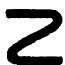
\includegraphics[keepaspectratio]{images/part001_a90573a3.jpg}}

PROPOSITION 8. Let \(f = \psi \circ g \circ \varphi\) be the canonical decomposition of a continuous mapping \(f: X \to Y\) , and let \(R\) denote the equivalence relation

\[
f (x) = f (y).
\]

Then the following three conditions are equivalent:

\begin{enumerate}
\def\labelenumi{\alph{enumi})}
\item
  \(g\) is a homeomorphism of \(\mathbf{X} / \mathbf{R}\) onto \(f(\mathbf{X})\) .
\item
  The image under \(f\) of every open set which is saturated with respect to \(\mathbf{R}\) is an open set in the subspace \(f(\mathbf{X})\) .
\item
  The image under \(f\) of every closed set which is saturated with respect to \(\mathbf{R}\) is a closed set in the subspace \(f(\mathbf{X})\) .
\end{enumerate}

For the condition b) {[}resp. c){]} expresses that the image under g of every open (resp. closed) set in X/R is an open (resp. closed) set in \(f(\mathbf{X})\) .

Example. Let X be a topological space, \((\mathbf{X}_{i})_{i\in I}\) a covering of X, Y the sum of the subspaces \(X_{v}\) of X; then there is a partition \((\mathbf{Y}_{i})_{i\in I}\) of Y into subspaces which are both open and closed, and for each \(i\in I\) there is a homeomorphism \(f_{i}:Y_{i}\to X_{i}\) . Let \(f:Y\to X\) be the continuous mapping which agrees with \(f_{i}\) on \(Y_{i}\) for each \(i\in I\) , and let R be the equivalence relation \(f(x)=f(y)\) ; the quotient space Y/R is thus obtained by ``pasting together'' the \(Y_{i}\) (§2, no. 5). Consider the bijection \(g:Y/R\to X\) associated with f; in general g is not a homeomorphism, as is shown by the example in which each \(X_{i}\) consists of a single point and X is not discrete. However, if the interiors of the \(X_{i}\) cover X, or if \((\mathbf{X}_{i})\) is a locally finite closed covering of X, then g is a homeomorphism: for if U is any open subset of Y which is saturated with respect to R, then for each \(i\in I\) the set

\[
f (\mathbf {U}) \cap \mathbf {X} _ {i} = f _ {i} (\mathbf {U} \cap \mathbf {Y} _ {i})
\]

is open in \(X_{i}\) , and the assertion follows from Proposition 3 of no. 1.

The following proposition gives a simple sufficient condition for \(g\) to be a homeomorphism:

PROPOSITION 9. Let \(f: \mathbf{X} \to \mathbf{Y}\) be a continuous surjection, and let \(\mathbf{R}\) denote the equivalence relation \(f(x) = f(y)\) . If there is a continuous section \(s: \mathbf{Y} \to \mathbf{X}\) associated with \(f\) (Set Theory, Chapter II, § 3, no. 8, Definition 11), then the mapping \(g: \mathbf{X} / \mathbf{R} \to \mathbf{Y}\) associated with \(f\) is a homeomorphism, and \(s\) is a homeomorphism of \(\mathbf{Y}\) onto the subspace \(s(\mathbf{Y})\) of \(\mathbf{X}\) .

For if \(\varphi: \mathbf{X} \to \mathbf{X} / \mathbf{R}\) is the canonical mapping, then \(g\) and \(\varphi \circ s\) are bijective, continuous and inverse to each other; likewise \(s\) and the restriction of \(f\) to \(s(\mathbf{Y})\) are bijective, continuous and inverse to each other.

If R is an equivalence relation on a topological space X and

\[
\varphi : \mathbf {X} \rightarrow \mathbf {X} / \mathbf {R}
\]

is the canonical mapping, a continuous section \(s: \mathbf{X} / \mathbf{R} \to \mathbf{X}\) associated with \(\varphi\) is also called a continuous section of \(\mathbf{X}\) with respect to \(\mathbf{R}\) (cf.~Set Theory, Chapter II, § 6, no. 2); the subspace \(s(\mathbf{X} / \mathbf{R})\) of \(\mathbf{X}\) is then homeomorphic to \(\mathbf{X} / \mathbf{R}\) . If we are given \(s(\mathbf{X} / \mathbf{R})\) , then \(s\) is uniquely determined; \(s(\mathbf{X} / \mathbf{R})\) is often called, by abuse of language, a (continuous) section of \(\mathbf{X}\) with respect to \(\mathbf{R}\) .

\pandocbounded{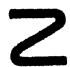
\includegraphics[keepaspectratio]{images/part001_feb98675.jpg}}

A continuous section of a topological space with respect to an equivalence relation need not exist (Exercise 12).

\subsection{QUOTIENT SPACE OF A SUBSPACE}

Let X be a topological space, A a subspace of X, R an equivalence relation on X, f the canonical map \(X \to X/R\) , g the restriction of f to A. The equivalence relation \(g(x) = g(y)\) on A is just the relation \(R_{A}\) induced by R on A (Set Theory R, § 5, no. 5). Let \(g = \psi \circ h \circ \varphi\) be the canonical decomposition of g, so that if j is the canonical injection of A into X we have a commutative diagram (*)

\begin{enumerate}
\def\labelenumi{(\Roman{enumi})}
\tightlist
\item
\end{enumerate}

\pandocbounded{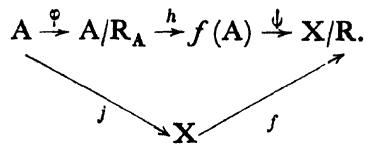
\includegraphics[keepaspectratio]{images/part001_6dc64900.jpg}}

PROPOSITION 10. The canonical bijection \(h: \mathbf{A} / \mathbf{R}_{\mathbf{A}} \to f(\mathbf{A})\) is continuous. Furthermore, the following three statements are equivalent:

\begin{enumerate}
\def\labelenumi{\alph{enumi})}
\item
  \(h\) is a homeomorphism.
\item
  Every open subset of A which is saturated with respect to \(R_{A}\) is the intersection with A of an open subset of X which is saturated with respect to R.
\item
  Every closed subset of A which is saturated with respect to \(R_{A}\) is the intersection with A of a closed subset of X which is saturated with respect to R.
\end{enumerate}

The first part of the proposition is immediate (no. 5). The second part follows from Proposition 8 of no. 5: if B is an open (resp. closed) subset of A which is saturated with respect to \(R_{A}\) , and \(g(B) = f(B)\) is the intersection with \(f(A)\) of an open (resp. closed) subset C of X/R, then B is the intersection with A of the open (resp. closed) subset \(\overline{f}(C)\)

of X, which is saturated with respect to R; and conversely, if B is the intersection with A of an open (resp. closed) subset D which is saturated with respect to R, then \(f(\mathbf{B})\) is the intersection of \(f(\mathbf{A})\) and \(f(\mathbf{D})\) , which is open (resp. closed) in X/R.

COROLLARY 1. If A is an open (resp. closed) subset of X which is saturated with respect to R, then the canonical mapping \(h: \mathrm{A}/\mathrm{R}_{\mathrm{A}} \rightarrow f(\mathrm{A})\) is a homeomorphism.

For if A is open (resp. closed) in X and saturated with respect to R, and if \(B \subset A\) is open (resp. closed) in A and saturated with respect to \(R_{A}\) , then B is open (resp. closed) in X and saturated with respect to R.

COROLLARY 2. If there is a continuous mapping \(u: \mathbf{X} \to \mathbf{A}\) such that \(u(x)\) is congruent to \(x \mod \mathbb{R}\) for each \(x \in \mathbf{X}\) , then \(f(\mathbf{A}) = \mathbf{X} / \mathbb{R}\) and the canonical mapping \(h: \mathbf{A} / \mathbb{R}_{\mathbf{A}} \to \mathbf{X} / \mathbb{R}\) is a homeomorphism.

Since each equivalence class mod R meets A, the canonical image of \(A/R_{A}\) in X/R is the whole of X/R; on the other hand, if U is open in A and is saturated with respect to \(R_{A}\) , it follows from the hypothesis that \(\overline{u}^{1}(U)\) is the set obtained by saturating U with respect to R; since u is continuous, \(\overline{u}^{1}(U)\) is open in X (§ 2, no. 1, Theorem 1). The corollary follows from this fact by virtue of Proposition 10.

Example. * Let R denote the equivalence relation \(x \equiv y \pmod{1}\) on the real line R (no. 4, Example) and let A denote the closed interval {[}0, 1{]}; A contains at least one point of each equivalence class mod R. The canonical mapping of \(\mathrm{A} / \mathbb{R}_{\mathbf{A}}\) onto the torus T is a homeomorphism; for if F is closed in A (and hence in R), in order to saturate F with respect to the relation R we have to take the union of the closed sets \(\mathrm{F} + n\) (for all \(n \in \mathbf{Z}\) ), which evidently form a locally finite family, so that their union is closed (§ 1, no. 5, Proposition 4); the assertion follows from this. We remark that \(\mathrm{A} / \mathbb{R}_{\mathbf{A}}\) is obtained by identifying the points 0 and 1 in A. *

\section{PRODUCT OF TOPOLOGICAL SPACES}

\subsection{PRODUCT SPACES}

DEFINITION 1. Given a family \((\mathbf{X}_{t})_{t\in I}\) of topological spaces, the product space of this family is the product set \(\mathbf{X} = \prod_{t\in I}\mathbf{X}_{t}\) with the topology which is the product of the topologies of the \(\mathbf{X}_{t}\) (§ 2, no. 3, Example 3). The spaces \(\mathbf{X}_{t}(t\in I)\) are called the factors of \(\mathbf{X}\) .

By virtue of § 2, no. 3, Proposition 4, the product topology on X has as a base the set B of finite intersections of sets of the form \(\overline{\mathrm{pr}}_{t}^{1}(\mathbf{U}_{t})\) , where \(U_{t}\) is open in \(X_{t}\) ; these sets are products \(\prod_{i\in I}A_{i}\) , where \(A_{i}\) is open in \(X_{t}\) for each \(i\in I\) and \(A_{i}=X_{t}\) for all but a finite number of indices. These sets will be called elementary sets.

If \(\mathfrak{B}_i\) is a base of the topology of \(X_i\) (for each \(i \in I\) ), it is clear that the elementary sets \(\prod_{i \in I} A_i\) such that \(A_i \in \mathfrak{B}_i\) for each index \(i\) such that \(A_i \neq X_i\) form another base of the product topology. The elementary sets of this type which contain a given point \(x \in X\) thus form a fundamental system of neighbourhoods of \(x\) ( \(\S 1\) , no. 3, Proposition 3).

If I is a finite set, the construction of the product topology from the topologies of the factors \(X_{i}\) is simpler: the elementary sets are just products \(\prod_{i\in I}A_{i}\) , where \(A_{i}\) is any open subset of \(X_{i}\) , for each \(i\in I\) (cf.~Exercise 9).

Examples. * The product \(\mathbf{R}^n\) of \(n\) spaces identical with the real line \(\mathbf{R}\) is called real number space of \(n\) dimensions; \(\mathbf{R}^2\) is also called the real plane (cf.~Chapter VI, § 1). Likewise, starting from the rational line \(\mathbf{Q}\) , we define the rational number space of \(n\) dimensions \(\mathbf{Q}^n\) (rational plane for \(n = 2\) ).

The topology of the space \(\mathbf{R}^n\) has as a base the set of all products of \(n\) open intervals in \(\mathbf{R}\) , which are called open boxes of \(n\) dimensions. The open boxes which contain a point \(x \in \mathbf{R}^n\) form a fundamental system of neighbourhoods of this point. Likewise the products of \(n\) closed intervals in \(\mathbf{R}\) are called closed boxes of \(n\) dimensions. The closed boxes to which \(x\) is interior also form a fundamental system of neighbourhoods of \(x\) . There are analogous results for \(\mathbf{Q}^n\) . *

PROPOSITION 1. Let \(f = (f_{i})\) be a mapping of a topological space \(Y\) into a product space \(X = \prod_{i \in I} X_{i}\) . Then \(f\) is continuous at a point \(a \in Y\) if and only if \(f_{i}\) is continuous at a for each \(i \in I\) .

Since \(f_{t} = \mathrm{pr}_{t} \circ f\) , this is just a particular case of Proposition 4 of §2, no. 3.

COROLLARY 1. Let \((\mathbf{X}_t)_{i \in \mathbf{I}}\) , \((\mathbf{Y}_t)_{i \in \mathbf{I}}\) be two families of topological spaces with the same set of indices. For each \(i \in \mathbf{I}\) , let \(f_i\) be a mapping of \(\mathbf{X}_t\) into \(\mathbf{Y}_t\) . In order that the product mapping \(f: (x_i) \to (f_i(x_i))\) of

\[
\prod_ {i \in I} X _ {i} \quad i n t o \quad \prod_ {i \in I} Y _ {i}
\]

should be continuous at a point \(a = (a_{i})\) it is necessary and sufficient that \(f_{i}\) is continuous at \(a_{i}\) for each \(\mathfrak{t} \in \mathbf{I}\) .

\(f\) can be written as \(x \to (f_{t}(\mathrm{pr}_{t}(x))\) , so that by Proposition 1 the condition is sufficient. Conversely, for each \(x \in I\) let \(g_{x}\) be the mapping of \(X_{x}\) into \(\prod_{i \in I} X_{i}\) such that \(\mathrm{pr}_{x}(g_{x}(x_{x})) = x_{x}\) and \(\mathrm{pr}_{t}(g_{x}(x_{x})) = a_{t}\) whenever \(i \neq x\) ; then \(g_{x}\) is continuous at the point \(a_{x}\) , by Proposition 1. Since \(f_{x} = \mathrm{pr}_{x} \circ f \circ g_{x}\) it follows that if \(f\) is continuous at \(a\) , then \(f_{x}\) is continuous at \(a_{x}\) .

COROLLARY 2. Let X, Y be two topological spaces. In order that a mapping \(f: \mathbf{X} \to \mathbf{Y}\) should be continuous it is necessary and sufficient that the mapping \(g: x \to (x, f(x))\) is a homeomorphism of X onto the graph G of \(f\) (considered as a subspace of the product space \(\mathbf{X} \times \mathbf{Y}\) ).

Since \(f = \mathrm{pr}_2 \circ g\) , the condition is sufficient. It is also necessary, for if \(f\) is continuous, then \(g\) is bijective and continuous (Proposition 1) and the inverse of \(g\) is the restriction of \(\mathrm{pr}_1\) to \(G\) , which is continuous (cf.~Set Theory, Chapter IV, § 2, no. 4, criterion CST 17).

PROPOSITION 2 (Associativity of topological products). Let \((\mathbf{X}_{\iota})_{\iota \in \mathbf{I}}\) be a family of topological spaces, \((\mathbf{J}_{\kappa})_{\kappa \in \mathbf{K}}\) a partition of the set I, and for each \(\kappa \in \mathbf{K}\) let \(\mathbf{X}_{\kappa}^{\prime} = \prod_{i\in \mathbf{J}_{\kappa}}\mathbf{X}_{\iota}\) be the product of the spaces \(\mathbf{X}_{\iota}\) for \(\iota \in \mathbf{J}_{\mathbf{K}}\) . Then the canonical mapping of the product space
